\documentclass{beamer}
\usepackage{graphicx}
\usepackage{amsmath}
\usepackage{lmodern}
\renewcommand{\familydefault}{\sfdefault}
\setbeamertemplate{navigation symbols}{}
\usecolortheme{default}
\usepackage{listings}
\usepackage{subfig}
\usepackage{fancyvrb}
\usepackage{tcolorbox,xcolor,tikz}
\tcbuselibrary{skins, breakable}

\renewcommand{\topfraction}{0.9}

\newenvironment{VerbatimIN}
 {\VerbatimEnvironment
  \begin{tcolorbox}[
    breakable,
    colback=lightgray,
    spartan
  ]%
  \begin{Verbatim}}
 {\end{Verbatim}\end{tcolorbox}}

 \newenvironment{VerbatimOUT}
 {\VerbatimEnvironment
  \begin{tcolorbox}[
    breakable,
    spartan
  ]%
  \begin{Verbatim}}
 {\end{Verbatim}\end{tcolorbox}}

\title{Mixed Effects Models - Day 1}
\subtitle{What are Mixed Effects Models, why and when should you use them, and what can you do with them}
\author{Marieke Wesselkamp \\ Department of Biometry and Environmental Systems Analysis \\ Albert-Ludwigs-University of Freiburg (Germany)}
\date{February 2023}

\begin{document}

\begin{frame}
  \titlepage
\end{frame}

\begin{frame}{Quote}
  \begin{center}
    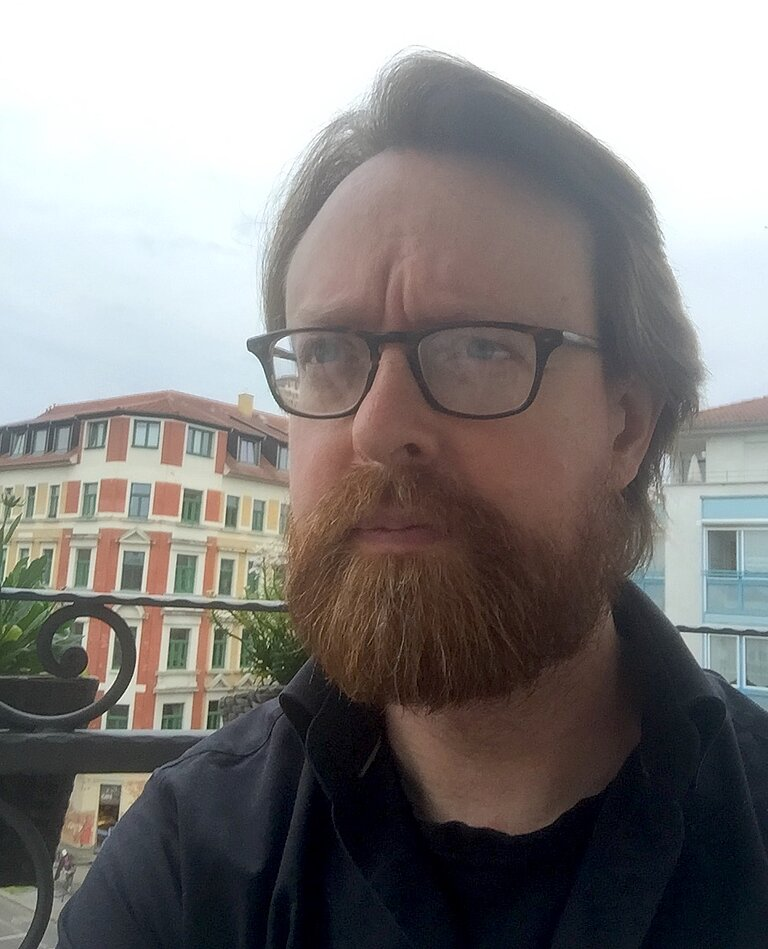
\includegraphics[width=0.4\textwidth]{lectures/day_1_intro_to_mems/figures/mcelreath2020.jpg}
    \\
    \bigskip
    \textit{"Rather start with a multilevel analysis and then realize it's unnecessary, than to overlook it."}
  \end{center}
\end{frame}

\begin{frame}{Soil Respiration Data}
  As ecologists, you might encounter this type of data:

\begin{figure}
    \centering
    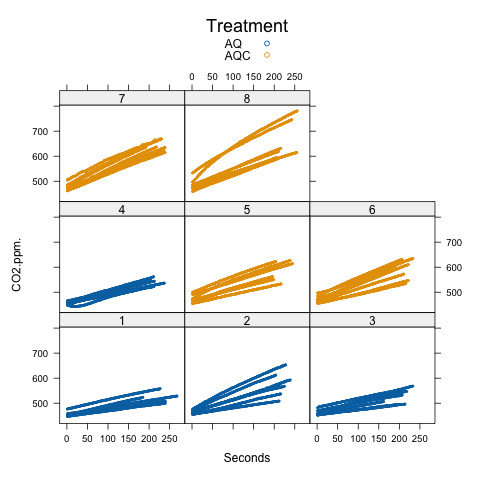
\includegraphics[width=0.5\linewidth]{lectures/day_1_intro_to_mems/figures/plot_1.png}
    \caption{Comparison of the soil respiration rate of two treatments, i.e. two forest stands with different vegetation composition. Source: Chair of Ecosystemphysiology Uni Freiburg}
\end{figure}

\end{frame}

\begin{frame}{Experimental Setup}
  \begin{itemize}
    \item 2 treatments, 8 chambers
    \item 7 measurements per chamber over two days
    \item Each measurement lasted at least 120 seconds
  \end{itemize}

  \begin{center}
    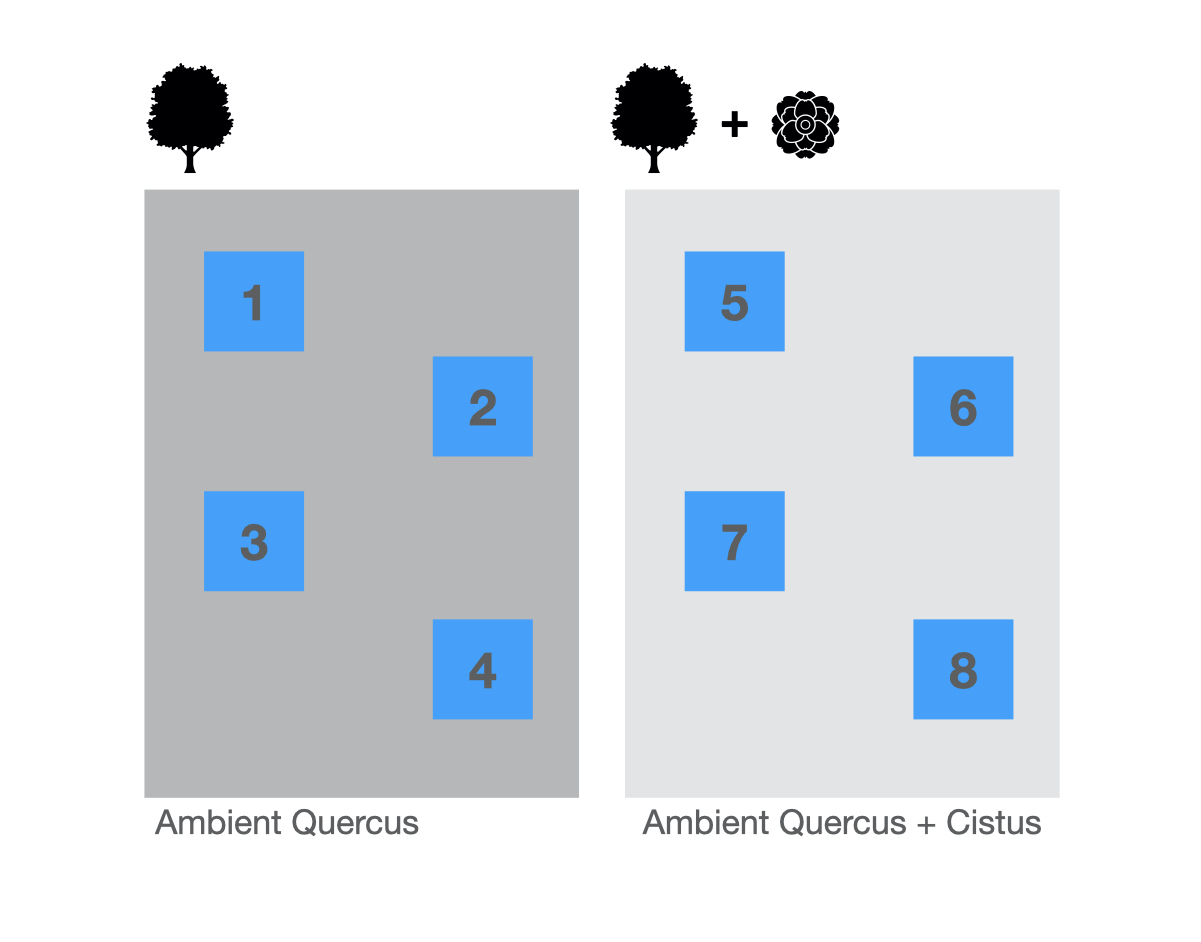
\includegraphics[width=0.7\textwidth]{lectures/day_1_intro_to_mems/figures/respiration.jpeg}
  \end{center}

\textbf{Hypothesis:} Higher soil respiration rate at the AQC stand.
\end{frame}

\begin{frame}
  \frametitle{}
  \begin{center}
    \huge\textbf{\textcolor{purple}{Hypothesis testing with non-independent data and avoidance of pseudo-replication}}
  \end{center}
\end{frame}

\begin{frame}[fragile]
\frametitle{{There is a Difference Between Two Treatments...}}
  \begin{columns}[onlytextwidth] % align columns at the top
    \begin{column}{0.44\textwidth}
      \begin{itemize}
        \item \textbf{20} measurements in each treatment
        \item \textbf{N = 40}
      \end{itemize}
    \end{column}
    \hspace{0.02\textwidth} % add small horizontal space
    \begin{column}{0.6\textwidth}
      \begin{center}
        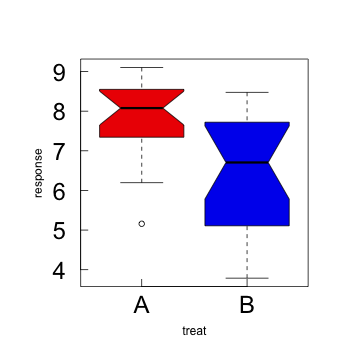
\includegraphics[width=0.8\textwidth]{lectures/day_1_intro_to_mems/figures/unnamed-chunk-5-1.png}
      \end{center}
    \end{column}
  \end{columns}
  \tiny
  \begin{VerbatimOUT}[numbers=left,numbersep=6pt]
Analysis of Variance Table

Response: response
          Df Sum Sq Mean Sq F value  Pr(>F)   
treat      1 17.660 17.6603  11.495 0.00164 **
Residuals 38 58.379  1.5363                   
---
Signif. codes:  0 '***' 0.001 '**' 0.01 '*' 0.05 '.' 0.1 ' ' 1      
  \end{VerbatimOUT}
\end{frame}

\begin{frame}[fragile]
\frametitle{Or is There?}
  \begin{columns}[onlytextwidth] % align columns at the top
    \begin{column}{0.44\textwidth}
  \begin{itemize}
    \item \textbf{10} measurements in each of two groups per treatment
    \item \textbf{N = 4}
  \end{itemize}
    \end{column}
    \hspace{0.02\textwidth} % add small horizontal space
    \begin{column}{0.6\textwidth}
      \begin{center}
        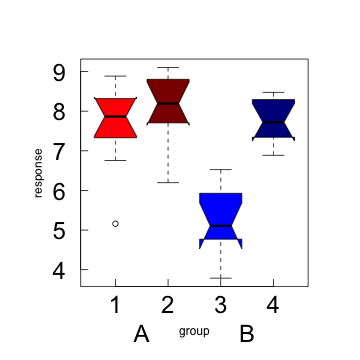
\includegraphics[width=0.8\textwidth]{lectures/day_1_intro_to_mems/figures/unnamed-chunk-7-1.png}
      \end{center}
    \end{column}
  \end{columns}
  \tiny
  \begin{VerbatimOUT}[numbers=left,numbersep=6pt]
Data: example_2
Models:
mod.2b: response ~ 1 + (1 | group)
mod.2a: response ~ treat + (1 | group)
       npar    AIC    BIC  logLik deviance  Chisq Df Pr(>Chisq)
mod.2b    3 119.92 124.98 -56.958   113.92                     
mod.2a    4 120.10 126.86 -56.051   112.10 1.8135  1     0.1781
  \end{VerbatimOUT}

\end{frame}

\begin{frame}{Pseudo-Replication}
  \begin{block}{Definition}
    Pseudo-replication occurs when one pretends to have more independent data points than there truly are. It matters for hypothesis testing because this is based on the degree of replication of independent data points \(N\). This sample size \(N\) gives rise to the degrees of freedom used in the calculation of test statistics and the p-value.
  \end{block}
\end{frame}

\begin{frame}{ANOVA Table}
  \resizebox{\linewidth}{!}{
  \begin{table}[h]
    \centering
    \footnotesize
    \begin{tabular}{lccccc}
      \hline
      Source & SS & df & MS & F & p \\
      \hline
      Treatment & SS\(_{\text{Treat}}\) & \(k_{\text{Treat}} - 1\) & SS\(_{\text{Treat}}\) / df\(_{\text{Treat}}\) & MS\(_{\text{Treat}}\) / MS\(_{\text{Res}}\) \\
      Residual & SS\(_{\text{Res}}\) & N - k & SS\(_{\text{Res}}\) / df\(_{\text{Res}}\) \\
      Total & SS\(_{\text{Total}}\) & N - 1 \\
      \hline
    \end{tabular}
  \end{table}}

  \vspace{0.5cm}

  \normalsize
  \textbf{Think about how the F-value and the p-value change when the number \(N\) (the replication = number of INDEPENDENT data points) changes.}
\end{frame}

\begin{frame}{Mixed Effect Models}
  \begin{enumerate}
      \item Mixed Effect Models are used to account for pseudo-replication and correlation (non-independence) of data points.
      \end{enumerate}
\end{frame}

\begin{frame}
  \frametitle{}
  \begin{center}
    \huge\textbf{\textcolor{purple}{Heterogeneity and missing information}}
  \end{center}
\end{frame}

\begin{frame}{What Do You Expect When You See This Plot?}
  \begin{center}
    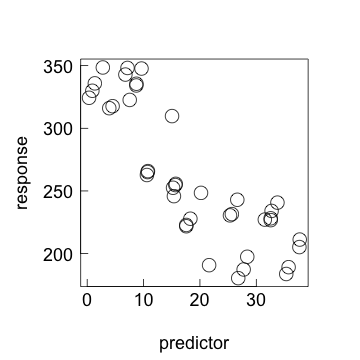
\includegraphics[width=0.6\textwidth]{lectures/day_1_intro_to_mems/figures/unnamed-chunk-8-1.png} % Replace with your figure path
  \end{center}
\end{frame}

\begin{frame}[fragile]
\frametitle{What Do You Expect When You See This Plot?}
\centering\textbf{The analysis using a Linear Model}
\vspace{0.7cm}

\begin{columns}[onlytextwidth] % align columns at the top
    \begin{column}{0.35\textwidth}
    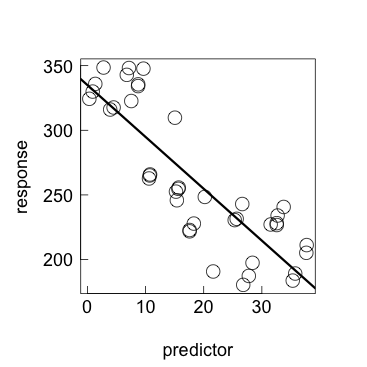
\includegraphics[width=0.999\textwidth]{lectures/day_1_intro_to_mems/figures/unnamed-chunk-11-1.png}
  \end{column}
    \hspace{0.0\textwidth} % add small horizontal space
\begin{column}{0.7\textwidth}
    \tiny
    \begin{VerbatimOUT}[numbers=left,numbersep=6pt]
Call:
lm(formula = y2 ~ x1, data = example_1)

Residuals:
    Min      1Q  Median      3Q     Max 
-57.449 -24.192  -1.917  24.017  51.347 

Coefficients:
            Estimate Std. Error t value Pr(>|t|)    
(Intercept) 334.9857     8.7161  38.433  < 2e-16 ***
x1           -4.0120     0.4021  -9.977 3.64e-12 ***
---
Signif. codes:  0 '***' 0.001 '**' 0.01 '*' 0.05 '.' 0.1 ' ' 1

Residual standard error: 29.06 on 38 degrees 
of freedom
Multiple R-squared:  0.7237,    Adjusted R-squared:  0.7164 
F-statistic: 99.54 on 1 and 38 DF,  p-value: 3.641e-12
    \end{VerbatimOUT}
    \end{column}
  \end{columns}

\end{frame}

\begin{frame}{What if You Knew That Some Data Points Group Together?}
  \begin{center}
    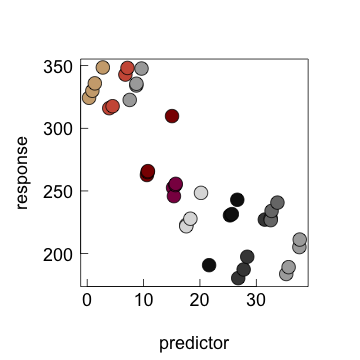
\includegraphics[width=0.6\textwidth]{lectures/day_1_intro_to_mems/figures/unnamed-chunk-12-1.png} % Replace with your figure path
  \end{center}
\end{frame}

\begin{frame}[fragile]
\frametitle{What if You Knew That Some Data Points Group Together?}

\textbf{The analysis using a Linear Mixed Effects Model}
\vspace{0.5cm}

\begin{columns}[onlytextwidth] % align columns at the top
    \begin{column}{0.4\textwidth}
    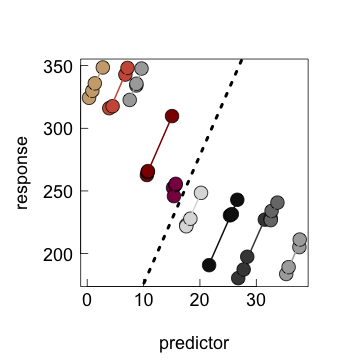
\includegraphics[width=0.999\textwidth]{lectures/day_1_intro_to_mems/figures/unnamed-chunk-14-1.png} % Replace 
  \end{column}
    \hspace{0.0\textwidth} % add small horizontal space
\begin{column}{0.6\textwidth}
    \tiny\begin{VerbatimOUT}[numbers=left,numbersep=6pt]
Linear mixed model fit by REML ['lmerMod']
Formula: y2 ~ x1 + (x1 | subject)

REML criterion at convergence: 260

Scaled residuals: 
     Min       1Q   Median       3Q      Max 
-2.67185 -0.42119  0.02881  0.49828  1.79544 

Random effects:
 Groups   Name        Variance  Std.Dev. Corr
 subject  (Intercept) 2.982e+04 172.6890     
          x1          1.114e-02   0.1055 1.00
 Residual             3.828e+00   1.9566     
Number of obs: 40, groups:  subject, 10

Fixed effects:
            Estimate Std. Error t value
(Intercept)   72.942     54.791   1.331
x1            10.275      0.245  41.944
optimizer (nloptwrap) convergence code: 0 (OK)
boundary (singular) fit: see ?isSingular
    \end{VerbatimOUT}
    \end{column}
  \end{columns}

\end{frame}


\begin{frame}[fragile]
\frametitle{Analysis Using a Linear Mixed Effects Model}
  \begin{itemize}
    \item A Mixed Effects Model is akin to modelling another variable.
  \end{itemize}
  \scriptsize
  \begin{VerbatimOUT}[numbers=left,numbersep=6pt]
Call:
lm(formula = y2 ~ x1 + x2, data = example_1)

Residuals:
    Min      1Q  Median      3Q     Max 
-4.2069 -0.9754 -0.1155  1.1961  4.0294 

Coefficients:
             Estimate Std. Error t value Pr(>|t|)    
(Intercept) 502.08553    1.85555  270.59   <2e-16 ***
x1           10.19269    0.15245   66.86   <2e-16 ***
x2           -6.07642    0.06425  -94.58   <2e-16 ***
---
Signif. codes:  0 '***' 0.001 '**' 0.01 '*' 0.05 '.' 0.1 ' ' 1

Residual standard error: 1.89 on 37 degrees 
of freedom
Multiple R-squared:  0.9989,    Adjusted R-squared:  0.9988 
F-statistic: 1.624e+04 on 2 and 37 DF,  p-value: < 2.2e-16
  \end{VerbatimOUT}
      
\end{frame}

\begin{frame}{Mixed Effect Models}
  \begin{enumerate}
      \item Mixed Effect Models are used to account for pseudo-replication and correlation (non-independence) of data points.
      \item Mixed Effects Models can provide better estimates for relationships in grouped data by capturing heterogeneity due to missing information that varies among groups.
      \end{enumerate}
\end{frame}

\begin{frame}
  \frametitle{}
  \begin{center}
    \huge\textbf{\textcolor{purple}{Modelling variances and variance components}}
  \end{center}
\end{frame}

\begin{frame}{}
  \begin{columns}[onlytextwidth] % align columns at the top
    \begin{column}{0.44\textwidth}
  \begin{itemize}
    \item \textbf{40} measurements of a response variable
  \end{itemize}
    \end{column}
    \hspace{0.02\textwidth} % add small horizontal space
    \begin{column}{0.6\textwidth}
      \begin{center}
        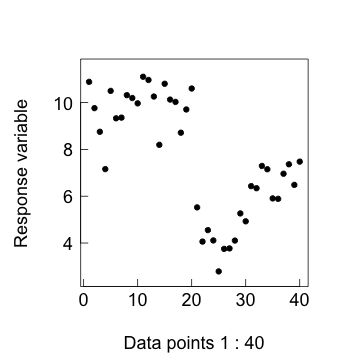
\includegraphics[width=0.9\textwidth]{lectures/day_1_intro_to_mems/figures/unnamed-chunk-16-1.png}
      \end{center}
    \end{column}
  \end{columns}
\end{frame}

\begin{frame}{}
  \begin{columns}[onlytextwidth] % align columns at the top
    \begin{column}{0.44\textwidth}
  \begin{itemize}
    \item the grand mean ...
  \end{itemize}
    \end{column}
    \hspace{0.02\textwidth} % add small horizontal space
    \begin{column}{0.6\textwidth}
      \begin{center}
        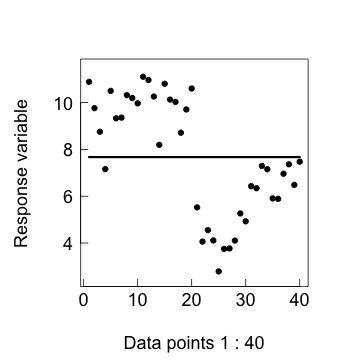
\includegraphics[width=0.9\textwidth]{lectures/day_1_intro_to_mems/figures/unnamed-chunk-18-1.png}
      \end{center}
    \end{column}
  \end{columns}
\end{frame}


\begin{frame}{}
  \begin{columns}[onlytextwidth] % align columns at the top
    \begin{column}{0.44\textwidth}
  \begin{itemize}
    \item ...and the variance around it
  \end{itemize}
    \end{column}
    \hspace{0.02\textwidth} % add small horizontal space
    \begin{column}{0.6\textwidth}
      \begin{center}
        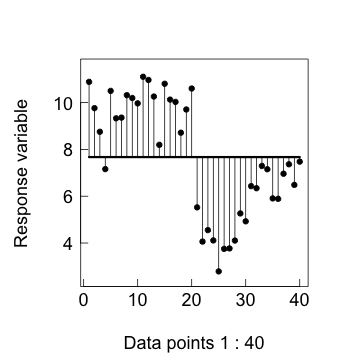
\includegraphics[width=0.9\textwidth]{lectures/day_1_intro_to_mems/figures/unnamed-chunk-19-1.png}
      \end{center}
    \end{column}
  \end{columns}
\end{frame}

\begin{frame}{}
  \begin{columns}[onlytextwidth] % align columns at the top
    \begin{column}{0.44\textwidth}
  \begin{itemize}
    \item but there are two treatments...
  \end{itemize}
    \end{column}
    \hspace{0.02\textwidth} % add small horizontal space
    \begin{column}{0.6\textwidth}
      \begin{center}
        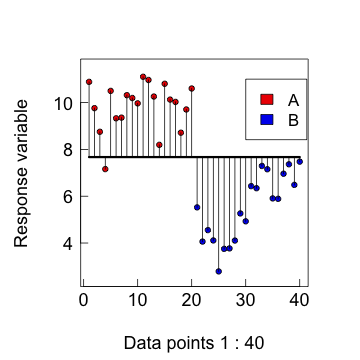
\includegraphics[width=0.9\textwidth]{lectures/day_1_intro_to_mems/figures/unnamed-chunk-20-1.png}
      \end{center}
    \end{column}
  \end{columns}
\end{frame}

\begin{frame}{}
  \begin{columns}[onlytextwidth] % align columns at the top
    \begin{column}{0.44\textwidth}
  \begin{itemize}
    \item ...with their means and the variances around them
  \end{itemize}
    \end{column}
    \hspace{0.02\textwidth} % add small horizontal space
    \begin{column}{0.6\textwidth}
      \begin{center}
        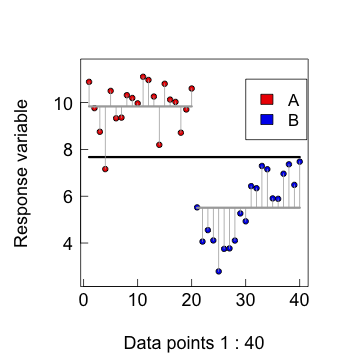
\includegraphics[width=0.9\textwidth]{lectures/day_1_intro_to_mems/figures/unnamed-chunk-22-1.png}
      \end{center}
    \end{column}
  \end{columns}
\end{frame}


\begin{frame}[fragile]
\frametitle{Variance in a Linear Model}

  \begin{columns}[onlytextwidth] % align columns at the top
    \begin{column}{0.6\textwidth}
    \tiny
    \begin{VerbatimOUT}[numbers=left,numbersep=6pt]
Analysis of Variance Table

Response: response
          Df  Sum Sq Mean Sq F value    Pr(>F)    
treatment  1 187.396 187.396  121.98 2.011e-13 ***
Residuals 38  58.379   1.536                      
---
Signif. codes:  0 '***' 0.001 '**' 0.01 '*' 0.05 
'.' 0.1 ' ' 1
    \end{VerbatimOUT}
    \end{column}
    \hspace{0.02\textwidth} % add small horizontal space
    \begin{column}{0.4\textwidth}
      \begin{center}
        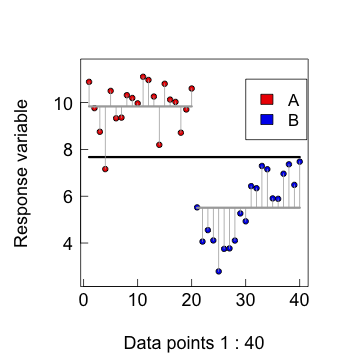
\includegraphics[width=0.999\textwidth]{lectures/day_1_intro_to_mems/figures/unnamed-chunk-22-1.png}
      \end{center}
    \end{column}
  \end{columns}
  \vspace{0.06\textwidth}
  \begin{itemize}
    \item \textbf{Variance\(_{total} = \text{Variance}_{treatment} + \text{Variance}_{residual}\)}
    \item \(245.775 = 187.396 + 58.379\)
  \end{itemize}
\end{frame}

\begin{frame}{Variances with Grouped Data}
  \begin{columns}[onlytextwidth] % align columns at the top
    \begin{column}{0.54\textwidth}
  \begin{itemize}
    \item Measurements in groups within each treatment...
  \end{itemize}    \end{column}
    \hspace{0.02\textwidth} % add small horizontal space
    \begin{column}{0.46\textwidth}
      \begin{center}
        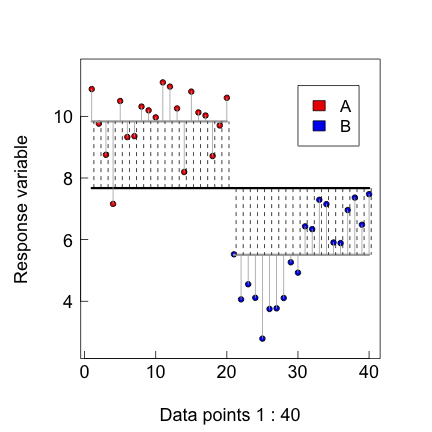
\includegraphics[width=0.999\textwidth]{lectures/day_1_intro_to_mems/figures/unnamed-chunk-23-1.png}
      \end{center}
    \end{column}
  \end{columns}
\end{frame}

\begin{frame}{Variances with Grouped Data}
  \begin{columns}[onlytextwidth] % align columns at the top
    \begin{column}{0.54\textwidth}
  \begin{itemize}
    \item ...and the \textbf{among-group variance} around treatment means (arrows)...
  \end{itemize}    \end{column}
    \hspace{0.02\textwidth} % add small horizontal space
    \begin{column}{0.46\textwidth}
      \begin{center}
        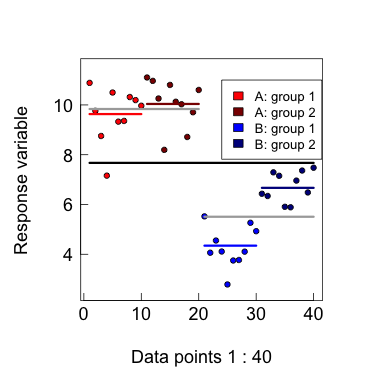
\includegraphics[width=0.999\textwidth]{lectures/day_1_intro_to_mems/figures/unnamed-chunk-24-1.png}
      \end{center}
    \end{column}
  \end{columns}
\end{frame}

\begin{frame}{Variances with Grouped Data}

\begin{columns}[onlytextwidth] 
    \begin{column}{0.54\textwidth}
  \begin{itemize}
    \item ...and the \textbf{within-group} or \textbf{residual variance} (coloured thin lines).
  \end{itemize}    \end{column}
    \hspace{0.02\textwidth} % add small horizontal space
    \begin{column}{0.46\textwidth}
      \begin{center}
        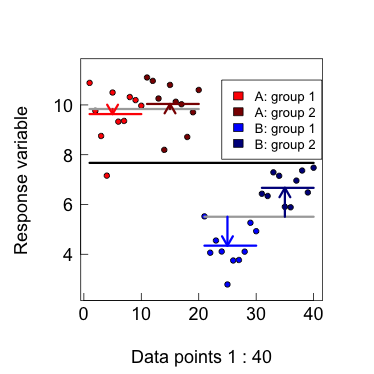
\includegraphics[width=0.999\textwidth]{lectures/day_1_intro_to_mems/figures/unnamed-chunk-25-1.png}
      \end{center}
    \end{column}
  \end{columns}
  
\end{frame}


\begin{frame}{Among-Group Variance}
  \begin{itemize}
    \item The \textbf{among-group} refers to the variance caused by different group means.
  \end{itemize}
  \begin{columns}[onlytextwidth] 
  \begin{column}{0.5\textwidth}
  \begin{center}
        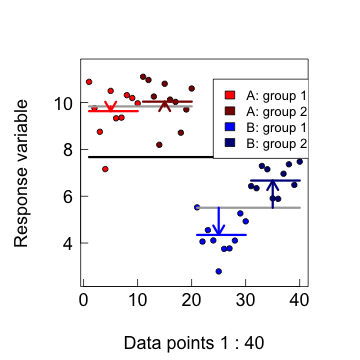
\includegraphics[width=0.999\textwidth]{lectures/day_1_intro_to_mems/figures/unnamed-chunk-27-1.png}
      \end{center}
      \[ \text{variance}_{\text{among}} = 1.462 \]
  \end{column}
    \hspace{0.02\textwidth} % add small horizontal space
    \begin{column}{0.5\textwidth}
      \begin{center}
        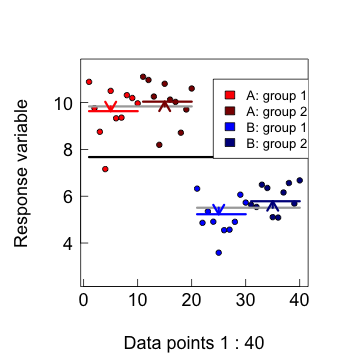
\includegraphics[width=0.999\textwidth]{lectures/day_1_intro_to_mems/figures/unnamed-chunk-28-1.png}
      \end{center}
        \[ \text{variance}_{\text{among}} = 0.147 \]
    \end{column}
  \end{columns}
  
\end{frame}

\begin{frame}{Within-Group Variance}
  \footnotesize{The \textbf{within-group} refers to the variance that is caused by differences within individual groups or levels.}
  
  \begin{columns}[onlytextwidth] 
  \begin{column}{0.5\textwidth}
  \begin{center}
        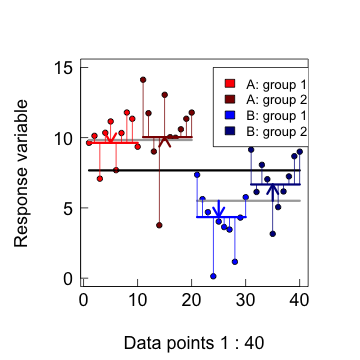
\includegraphics[width=0.999\textwidth]{lectures/day_1_intro_to_mems/figures/unnamed-chunk-30-1.png}
      \end{center}
      \[ \text{variance}_{\text{within}} = 0.875 \]
  \end{column}
    \hspace{0.02\textwidth} % add small horizontal space
    \begin{column}{0.5\textwidth}
      \begin{center}
        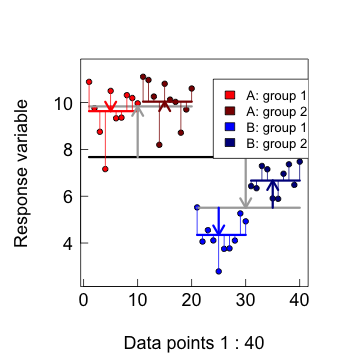
\includegraphics[width=0.999\textwidth]{lectures/day_1_intro_to_mems/figures/unnamed-chunk-36-1.png}
      \end{center}
        \[ \text{variance}_{\text{within}} = 0.1723 \]
    \end{column}
  \end{columns}

\end{frame}



\begin{frame}{Intra-Group Correlation (ICC)}
  \begin{itemize}
    \item The \textbf{intra-group correlation ICC} is the ratio of the among-group variance to the total variance.
  \end{itemize}

  \begin{equation*}
    ICC = \frac{\text{variance}_{\text{among}}}{\text{variance}_{\text{among}} + \text{variance}_{\text{within}}}
  \end{equation*}
\end{frame}

\begin{frame}{Adjusted Intra-Group Correlation}
  \begin{itemize}
    \item The \textbf{intra-group correlation ICC}  ranges between 0 and 1, providing various insights:
    \begin{itemize}
      \item It shows how similar data points from the same group are compared to data points from different groups.
      \item It can be interpreted as the expected correlation between two randomly drawn data points from the same group.
      \item It helps estimate effective sample size: 
      \[
      N_{\text{eff}} = \frac{N_{\text{total}} \cdot N_{\text{group}}}{1 + (N_{\text{group}} - 1) \cdot ICC}
      \]
    \end{itemize}
  \end{itemize}
\end{frame}

\begin{frame}[fragile]
\frametitle{Adjusted Intra-Group Correlation}
  \footnotesize{Accounting for \textbf{only} among-group differences changes the variances and the ICC}
  \tiny
    \begin{VerbatimIN}[numbers=left,numbersep=6pt]
lmer(formula = response ~ treatment + (1 | group))  # LEFT
lmer(formula = response ~ 1 + (1 | group))          # RIGHT
    \end{VerbatimIN}
  \footnotesize
  \begin{columns}[onlytextwidth] 
  \begin{column}{0.5\textwidth}
    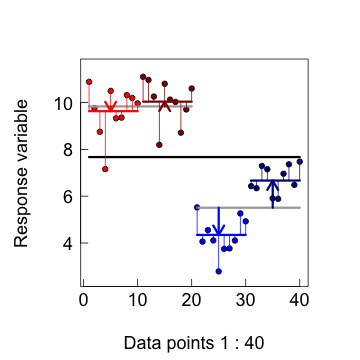
\includegraphics[width=0.8\textwidth]{lectures/day_1_intro_to_mems/figures/unnamed-chunk-32-1.png}    
  \end{column}
    \hspace{0.02\textwidth} % add small horizontal space
    \begin{column}{0.5\textwidth}
      \centering
        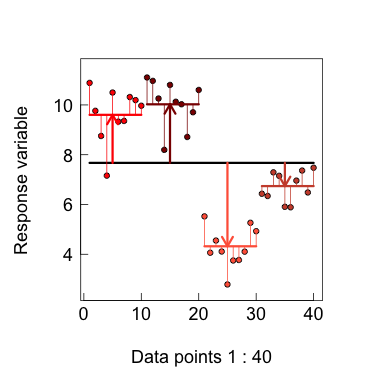
\includegraphics[width=0.7\textwidth]{lectures/day_1_intro_to_mems/figures/unnamed-chunk-34-1.png}
    \end{column}
  \end{columns}

  \begin{columns}[onlytextwidth] 
  \begin{column}{0.5\textwidth}
  \textbf{with} treatment \\
  \begin{itemize}
      \item $\text{variance}_{\text{among}} = 1.463$
      \item $\text{variance}_{\text{among}} = 0.766$ 
      \item ICC =  0.656
  \end{itemize}

  \end{column}
    \hspace{0.02\textwidth} % add small horizontal space
    \begin{column}{0.5\textwidth}
    \textbf{without} treatment
    \begin{itemize}
      \item $\text{variance}_{\text{among}} = 7.196$
      \item $\text{variance}_{\text{among}} = 0.766$ 
      \item ICC =   0.904
  \end{itemize}
    \end{column}
  \end{columns}

\end{frame}

\begin{frame}{Conclusion}
  \begin{enumerate}
      \item Mixed Effect Models are used to account for pseudo-replication and correlation (non-independence) of data points.
      \item Mixed Effects Models can provide better estimates for relationships in grouped data by capturing heterogeneity due to missing information that varies among groups.
      \item Mixed Effects Models allow the estimation of the variances at different levels of the data.
    \end{enumerate}
\end{frame}


\begin{frame}
  \frametitle{}
  \begin{center}
    \huge\textbf{\textcolor{purple}{Quantification of Group-Level Parameters}}
  \end{center}
\end{frame}


\begin{frame}{Quantification of Group-Level Parameters}

\begin{columns}[onlytextwidth] 
  \begin{column}{0.4\textwidth}
  \begin{itemize}
      \item in gray: treatment effects = fixed effects parameters
      \item coloured: group effects = random effects parameters
  \end{itemize}
    \end{column}
    \hspace{0.02\textwidth} % add small horizontal space
    \begin{column}{0.5\textwidth}
      \begin{center}
        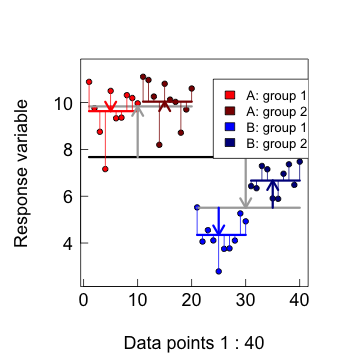
\includegraphics[width=0.9\textwidth]{lectures/day_1_intro_to_mems/figures/unnamed-chunk-35-1.png}
      \end{center}
    \end{column}
  \end{columns}
  
  \begin{itemize}
    \item \textbf{Fixed Effects Parameters} provide the \textbf{population average}, e.g., how much a treatment differs from a grand mean or how, on average, the response changes with a covariate.
    \item \textbf{Random Effects Parameters} represent the \textbf{group-specific deviations} from that average population mean or slope.
  \end{itemize}
  
\end{frame}

\begin{frame}[fragile]
\frametitle{Group-Level Parameters}

\textbf{Random Intercepts}

\begin{columns}[onlytextwidth] 
  \begin{column}{0.5\textwidth}
  \scriptsize
  \begin{VerbatimOUT}[numbers=left,numbersep=6pt]
$group
  (Intercept)
1  -0.2031451
2   0.2031451
3  -1.1613079
4   1.1613079

with conditional variances 
for "group"      
  \end{VerbatimOUT}
  \begin{VerbatimOUT}[numbers=left,numbersep=6pt]
treatmentA treatmentB 
  9.836181   5.507260  
  \end{VerbatimOUT}
      \end{column}
    \hspace{0.02\textwidth} % add small horizontal space
    \begin{column}{0.5\textwidth}
      \begin{center}
        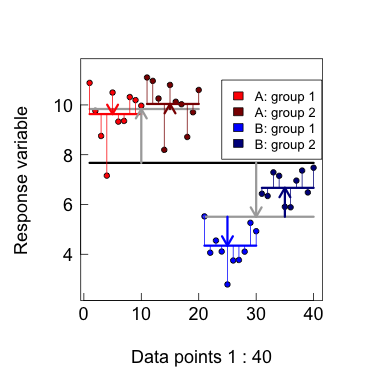
\includegraphics[width=0.9\textwidth]{lectures/day_1_intro_to_mems/figures/unnamed-chunk-37-1.png}
      \end{center}
    \end{column}
  \end{columns}

\end{frame}


\begin{frame}[fragile]
\frametitle{Group-Level Parameters}

\textbf{Random intercepts and random slopes}

\begin{columns}[onlytextwidth] 
  \begin{column}{0.5\textwidth}
  \scriptsize
  \begin{VerbatimOUT}[numbers=left,numbersep=6pt]
$subject
   (Intercept)          x1
1    247.69897  0.15137981
2    200.13944  0.12231407
3    172.20003  0.10523907
4     81.20556  0.04962831
5     19.86128  0.01213811
6    -31.53238 -0.01927083
7   -102.41808 -0.06259223
8   -165.97361 -0.10143383
9   -175.02052 -0.10696279
10  -246.16068 -0.15043969

with conditional variances 
for "subject" 

(Intercept)          x1 
   72.94195    10.27548 
  \end{VerbatimOUT}
      \end{column}
    \hspace{0.02\textwidth} % add small horizontal space
    \begin{column}{0.5\textwidth}
      \begin{center}
        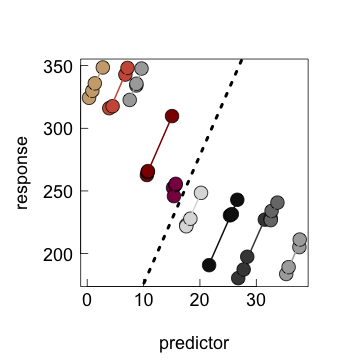
\includegraphics[width=0.9\textwidth]{lectures/day_1_intro_to_mems/figures/unnamed-chunk-38-1.png}
      \end{center}
    \end{column}
  \end{columns}

\end{frame}


\begin{frame}{To Summarize}

  \begin{enumerate}
      \item Mixed Effect Models are used to account for pseudo-replication and correlation (non-independence) of data points.
      \item Mixed Effects Models can provide better estimates for relationships in grouped data by capturing heterogeneity due to missing information that varies among groups.
      \item Mixed Effects Models allow the estimation of the variances at different levels of the data.
          \item They let one estimate the group-specific parameters (intercept, slope, interactions).
    \end{enumerate}
    
 \end{frame}


\begin{frame}
  \frametitle{}
  \begin{center}
    \huge\textbf{\textcolor{purple}{Break!}}
  \end{center}
\end{frame}

\begin{frame}{What are Grouped Data?}
  \begin{itemize}
    \item \textbf{Temporal}: repeated measurements of the same unit over time, e.g., monthly counts of animals in a population or measurements over a fish's lifespan.
    \item \textbf{Spatial}: samples taken at locations close together, e.g., on a forest site or a meadow or in one country.
    \item \textbf{Individual}: repeated measurements at one individual, e.g., a tree whose moss cover is measured on each of the sides of the compass.
    \item \textbf{Phylogenetic}: measurements belong together because they come from the same species or family.
  \end{itemize}
\end{frame}

\begin{frame}{Forms of Grouped Data}
\begin{columns}[onlytextwidth] 
  \begin{column}{0.5\textwidth}
      \begin{center}
    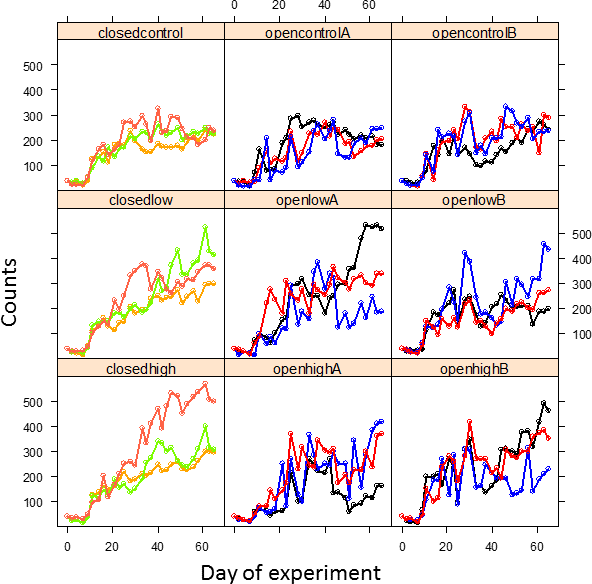
\includegraphics[width=0.99\textwidth]{lectures/day_1_intro_to_mems/figures/counts.png} % Replace with your figure path
  \end{center}
      \end{column}
    \hspace{0.02\textwidth} % add small horizontal space
    \begin{column}{0.5\textwidth}
       36 counts over 72 days of adult mites per each of 27 population in 9 treatments. What is the grouping variable? 
    \end{column}
\end{columns}

  \end{frame}

\begin{frame}{Forms of Grouped Data}
  \begin{columns}[onlytextwidth] 
  \begin{column}{0.5\textwidth}
      \begin{center}
    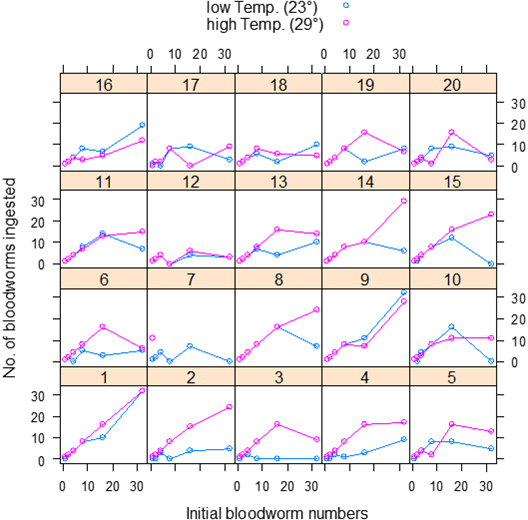
\includegraphics[width=0.99\textwidth]{lectures/day_1_intro_to_mems/figures/bloodworms.png} % Replace with your figure path
  \end{center}
      \end{column}
    \hspace{0.02\textwidth} % add small horizontal space
    \begin{column}{0.5\textwidth}
        Counts of prey eaten over 6 initial prey densities by each of 20 fish at two different temperatures. What is the grouping variable?  
    \end{column}
\end{columns}  \end{frame}


\begin{frame}{Forms of Grouped Data}
  \begin{itemize}
    \item There can be several grouping variables of different forms and a hierarchy with multiple levels. 
  \end{itemize}
  \begin{center}
    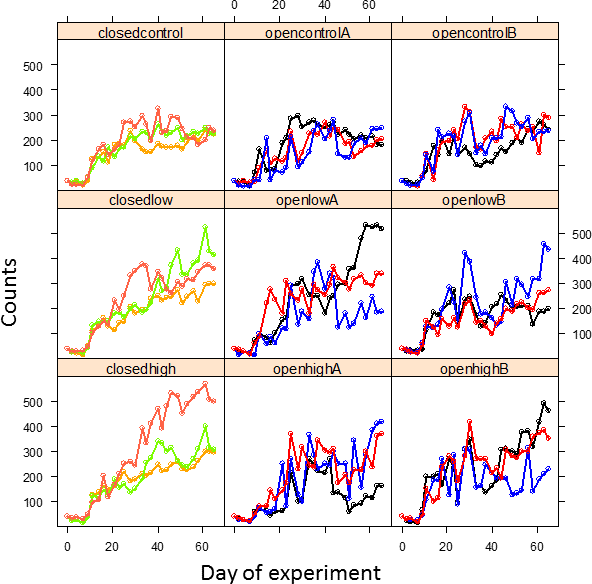
\includegraphics[width=0.5\textwidth]{lectures/day_1_intro_to_mems/figures/counts.png} % Replace with your figure path
  \end{center}
      e.g. beetle counts measured over time in 5 single plots (each line a plot) in four different regions (each panel a region). Grouping occurs within plot (over years) but also within a region (over plots). Plot is nested within region. 
\end{frame}



\begin{frame}{Design of Experiments: Randomised Blocked}
  \begin{itemize}
    \item Definition: The treatment areas of all treatment combinations are combined in one block. This block is then replicated. The treatments are randomly assigned to the surfaces within a block.
  \end{itemize}
  \begin{center}
    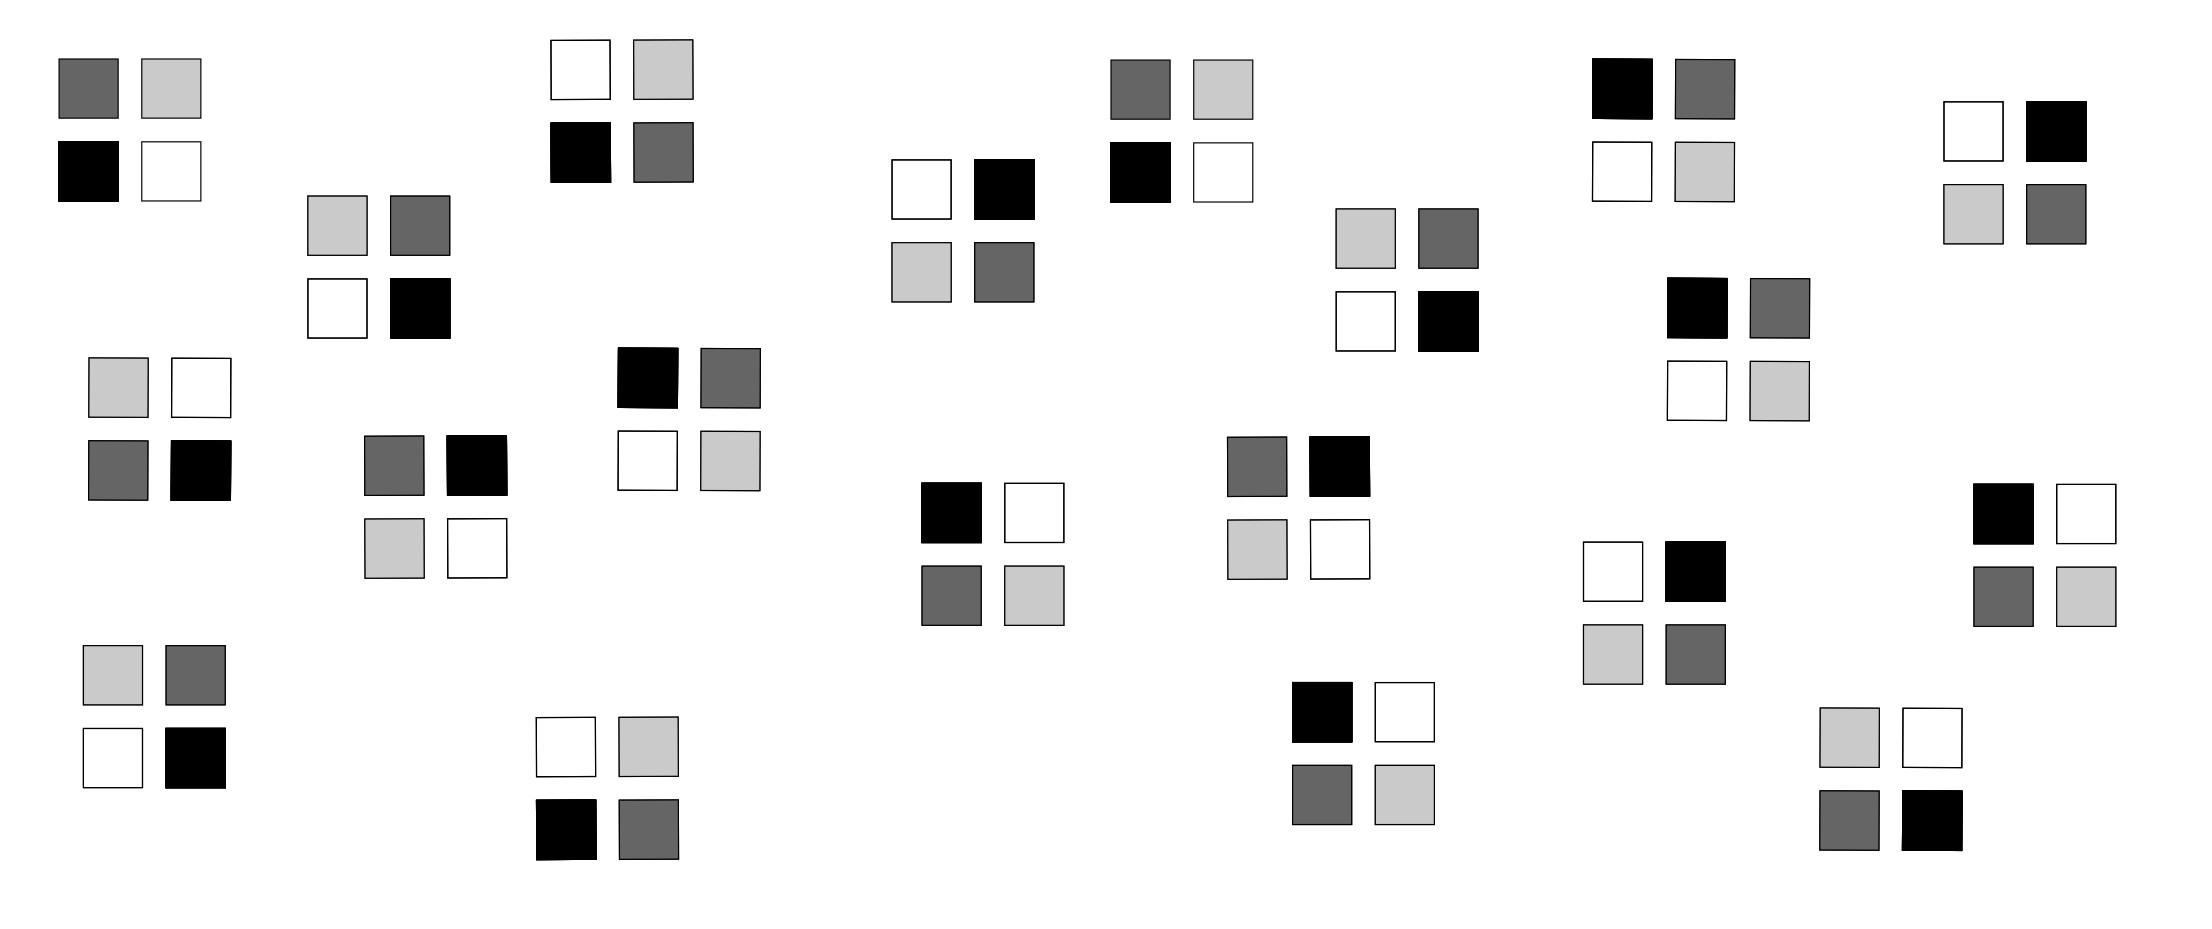
\includegraphics[width=0.4\textwidth]{lectures/day_1_intro_to_mems/figures/randomisedblockfig.png}
  \end{center}
\end{frame}

\begin{frame}{Design of Experiments: Nested}
  \begin{itemize}
    \item Definition: Several measurements are performed within an experimental unit, either in parallel (multiple objects side-by-side) or sequentially over time (repeated measurements).
  \end{itemize}
  \begin{center}
    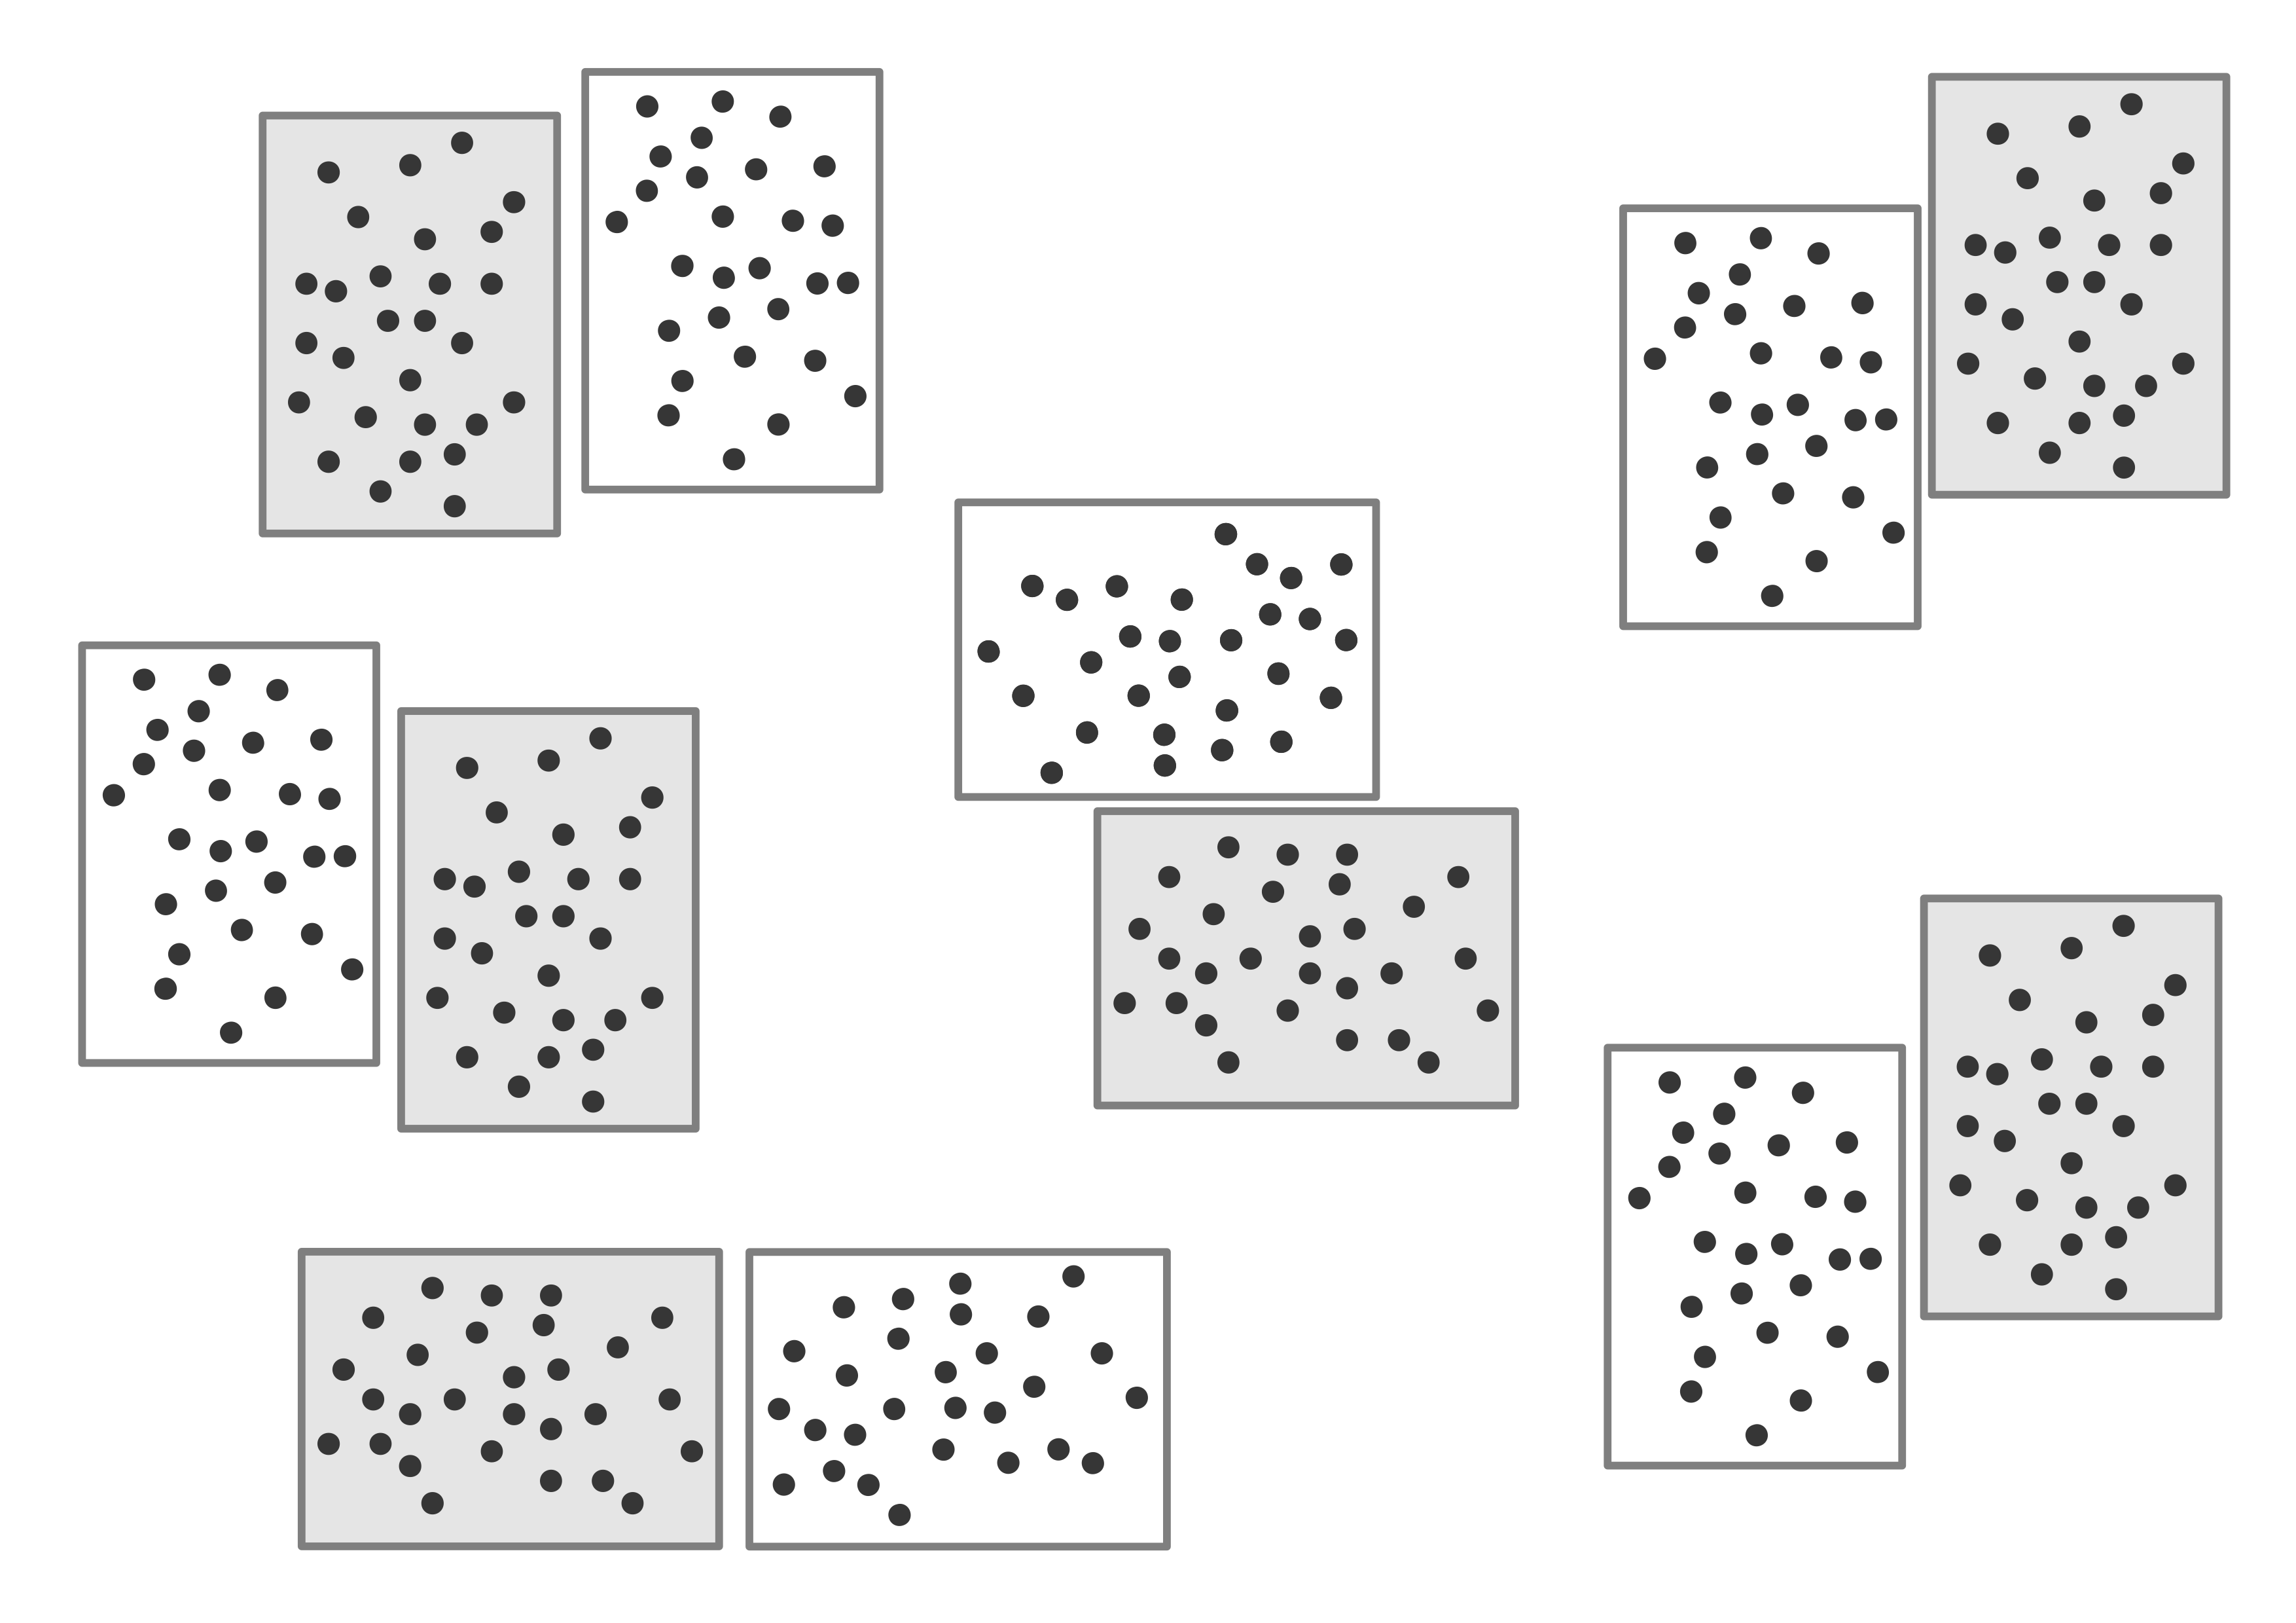
\includegraphics[width=0.4\textwidth]{lectures/day_1_intro_to_mems/figures/nesteddesign.png}
  \end{center}
\end{frame}

\begin{frame}{Design of Experiments: Split-Plot}
  \begin{itemize}
    \item Definition: The different levels of a treatment are applied within each level of another treatment.
  \end{itemize}
  \begin{center}
    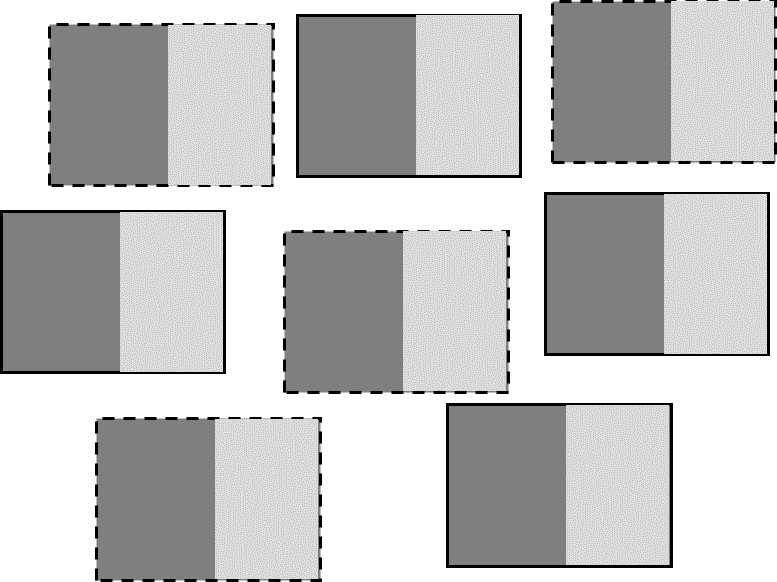
\includegraphics[width=0.4\textwidth]{lectures/day_1_intro_to_mems/figures/splitplot.png}
  \end{center}
\end{frame}

\begin{frame}{Random vs. Fixed Effects}
  \begin{itemize}
    \item "The main distinction between a fixed and a random effect is whether you're measuring a few specific instances of interest in themselves (fixed) or a few randomly chosen instances interesting only as representatives of a population (random)." — Brian McGill on Dynamic Ecology
  \end{itemize}
\end{frame}

\begin{frame}{Random vs. Fixed Effects}

some PRACTICAL guidelines of what is Fixed and what is Random (after M. Crawley: The R-Book)

  \begin{itemize}
    \item Am I interested in the effect sizes? Yes = Fixed
    \item Do the factor levels come from a population of levels? Yes = Random
    \item Are there enough levels of the grouping variable to estimate a variance (min. 5 or 7)? No = Fixed
    \item Are the factor levels of the group informativ? Yes = Fixed 
    \item Or are the factor levels just arbitrary labels? Yes = Random
    \item Am I interested in inference about the effect distribution? Yes = Random 
    
  \end{itemize}
\end{frame}


\begin{frame}{Choosing Random and Fixed Effects}
  \begin{itemize}
    \item Choose random and fixed effects \textbf{before} data acquisition.
    \item Otherwise, you may not be able to achieve what you want with your Mixed Effects Model because you gathered the wrong or insufficient data with an inefficient design.
  \end{itemize}

  More about this distinction and how to choose random effects during exercises and discussions in the exercises.
  
\end{frame}

\begin{frame}{Some Sources for Further Reading}
  \begin{itemize}
    \item \href{https://stats.stackexchange.com/questions/4700/what-is-the-difference-between-fixed-effect-random-effect-and-mixed-effect-mode/4702#4702}{What is the difference between fixed-effect, random-effect, and mixed-effect models?}
    \item \href{https://dynamicecology.wordpress.com/2015/11/04/is-it-a-fixed-or-random-effect/}{Is it a fixed or random effect?}
    \item \href{https://gkhajduk.github.io/2017-03-09-mixed-models/}{Gabriela Hajduk on Mixed Effects Models}
  \end{itemize}
\end{frame}

\begin{frame}{More Sources for Mixed Effects Models}
ONLINE
  \begin{itemize}
    \item APES - statistical advice site of the biometry department: 
    \item introductionary workshop by Gabriela Hajduk:
    \item FAQ list by B Bolker, co-developer of lme4 package: here
    \item cheat sheet for lmer: here
    \item very basic Wikipedia entry: here
  \end{itemize}

BOOKS
  \begin{itemize}
    \item Zuur et al. Mixed Effects Models and Extensions in Ecology with R link
    \item Pinheiro & Bates Mixed-Effects Models in S and S-PLUS link
    \item Crawley The R-Book, chapters 11 & 19 (pdfs throughout the WWW) link
  \end{itemize}
  
\end{frame}

\begin{frame}{Final Note on Terminology}
  \footnotesize{
    what I will call Mixed Effects Models in this course comprises a number of models that all incorporate mixed and random effects (therefore “mixed”) but come under different names and sometimes use different estimation techniques. Nested, repeated-measurements and split-plot ANOVAs are based on ordinary least-square techniques and are used for balanced, gaussian data. They are thus a special case of the more general Mixed Effects Models which are often also termed Multi-level or Hierarchical Models (because of the hierarchy of multiple levels in the data). In other disciplines outside the environmental sciences Mixed Effects Models come under names such as Panel Data Models or Subject-Level Models for reasons that should be obvious by now. All have in common the grouping of data into plots, sites, regions, populations, species, family, subjects, individuals, classes etc. but often differ in the used terminolgy. E.g. what I call the intra-group correlation is often termed the intra-class correlation or, in behavioural ecology, repeatability because it gives a measure of how consistent differences in behaviour among individuals are. 
  }
\end{frame}

\begin{frame}{Recapitulation Day 1}
After today you should know and understand what the \textbf{bold} terms and concepts mean
  \begin{itemize}
    \item Mixed Effects Models contain \textbf{fixed} and \textbf{random} effects.
    \item Mixed Effects Models are statistical tools to analyze \textbf{grouped data} of various forms.
    \item They account for (1) \textbf{non-independence, pseudo-replication, and correlation} of data points...
    \item ... and can do much more: (2) capture effects of \textbf{missing} information, (3) quantify \textbf{among-group} and \textbf{within-group} variances, and estimate \textbf{group-level} parameters.
  \end{itemize}
  Today Exercise: reading, discussion, exercises on Random Effects
  
\end{frame}

\end{document}